\documentclass[11pt]{article}
\usepackage{homework}

\classname{361}
\homeworknum{3}



\begin{document}

% Environments

\newcommand{\state}[2]{\begin{statement}{#1} #2 \end{statement}}
\newcommand{\prob}[2]{\begin{problem}{#1} #2 \end{problem}}
\newcommand{\subprob}[1]{\begin{subproblem} #1 \end{subproblem}}
\newcommand{\sol}[1]{\begin{solution} #1 \end{solution}}
\newcommand{\fig}[2]{\begin{figure} \centering #2  \label{#1} \end{figure}}

\newcommand{\makebib}{
	\vfill
	\color{black}
	\nocite{*}
	\bibliography{references}{}
	\bibliographystyle{lucas_unsrt}
}
	

% Implication

\newcommand{\qwhere}{\quad \text{where} \quad}
\newcommand{\qimplies}{\quad \implies \quad}
\newcommand{\impliesq}{\implies \quad}



% Brackets

\newcommand{\paren}[1]{\left( #1 \right)}
\newcommand{\brac}[1]{\left[ #1 \right]}
\newcommand{\curly}[1]{\left\{ #1 \right\}}


% Greek

\newcommand{\alp}{\alpha}
\newcommand{\bet}{\beta}
\newcommand{\gam}{\gamma}
\newcommand{\del}{\delta}
\newcommand{\eps}{\epsilon}
\newcommand{\zet}{\zeta}
\newcommand{\tht}{\theta}
\newcommand{\kap}{\kappa}
\newcommand{\lam}{\lambda}
\newcommand{\sig}{\sigma}
\newcommand{\ups}{\upsilon}
\newcommand{\omg}{\omega}

\newcommand{\Gam}{\Gamma}
\newcommand{\Del}{\Delta}
\newcommand{\Tht}{\Theta}
\newcommand{\Lam}{\Lambda}
\newcommand{\Sig}{\Sigma}
\newcommand{\Omg}{\Omega}


% Text

\newcommand{\where}{\text{where }}

% Problem 1

\newcommand{\Hint}{H_\text{int}}
\newcommand{\ddcx}{\dd[3]{x}}
\newcommand{\psib}{\bar{\psi}}

\newcommand{\mh}{m_h}
\newcommand{\mmu}{m_\mu}
\newcommand{\me}{m_e}
\newcommand{\ma}{m_a}

\newcommand{\aexpt}{a_\text{expt.}}
\newcommand{\aQED}{a_\text{QED}}
\renewcommand{\GeV}{\giga\electronvolt}

\newcommand{\gamt}{\gam^5}


\state{Bloch's theorem}{	\label{1}
	Prove Bloch's theorem by operating with the translation operator on $H \psi$ and using the periodic symmetry of the potential.  Show furthermore that $\TR \TRp = \TRp \TR = \TRpRp$; the translation operators commute with themselves.
}

\sol{
	Bloch's theorem is given by (8.6) of Ashcroft \& Mermin:
	\eq{
		\psirpR = e^{i \vk \vdot \vR} \psir.
	}
	Additionally, $H \psir$ is given by (4.1):
	\eq{
		H \psir = \paren{ -\frac{\hbar^2}{2 m} \laplacian + \Ur } \psir.
	}
	
	According to (4.5) in the lecture notes, the action of the translation operator is $\TR \fr = \frpR$.  Operating on $H \psi$ yields~\cite[p.~134]{Ashcroft}
	\al{
		\TR (H \psi) &= \HrpR \psirpR \\
		&= \paren{ -\frac{\hbar^2}{2 m} \laplacian + \UrpR } \psirpR \\
		&= \paren{ -\frac{\hbar^2}{2 m} \laplacian + \Ur } \psirpR \\
		&= \Hr \psirpR \\
		&= H \TR \psi,
	}
	since $\Ur = \UrpR$ for all $\vR$ in a Bravais lattice according to p.~35 of the lecture notes.  Thus we have shown
	\eq{
		\TR H = H \TR;
	}
	that is, $H$ and $\TR$ commute.
	
	Note also that
	\eq{
		\TR \TRp \fr = \TR f(\vr + \vR')
		= f(\vr + \vR' + \vR)
		= f(\vr + \vR + \vR')
		= \TRp f(\vr + \vR)
		= \TRp \TR \fr
	}
	and that
	\eq{
		\TRpRp \fr = f(\vr + \vR + \vR'),
	}
	so we have shown that
	\eq{ \eqqed{
		\ans{ \TR \TRp = \TRp \TR = \TRpRp. } \qedhere
	}}
	
	Since $H$ and $\TR$ commute and the $\TR$s commute with each other, they can be simultaneously diagonalized.  We can apply (4.8) of the lecture notes:
	\aln{ \label{eigenvals}
		H \psi &= E \psi, &
		\TR \psi &= \cR \psi.
	}
	Now applying what we have just proven about the $\TR$s,
	\eqn{cRs}{
		\cR \cRp \psi = \TR \TRp \psi
		= \TRpRp \psi
		= \cRpRp \psi
		\qimplies
		\cR \cRp = \cRpRp.
	}
	From Ashcroft \& Mermin~(4.1), any position vector $\vR$ on the Bravais lattice can be written
	\eq{
		\vR = \nq \vaq + \nw \vaw + \nee \vae,
	}
	where the $\nii$ are integers.  So using Eq.~\refeq{cRs}, we can write
	\eqn{thing1}{
		\cR = c(\nq \vaq + \nw \vaw + \nee \vae)
		= c(\nq \vaq) c(\nw \vaw) c(\nee \vae)
		= c(\vaq)^{\nq} c(\vaw)^{\nw} c(\vae)^{\nee}.
	}
	We define the numbers $\ki$ such that (4.10) of the lecture notes is satisfied:
	\eq{
		\cai = e^{2\pi i \ki},
	}
	where $\vai$ are the primitive vectors of the lattice.  Applying this to Eq.~\refeq{thing1},
	\eqn{thing1.b}{
		\cR = (e^{2\pi i \kq})^{\nq} (e^{2\pi i \kw})^{\nw} (e^{2\pi i \ke})^{\nee}
		= e^{2\pi i (\kq \nq + \kw \nw + \ke \nee)}
		= e^{i \vk \vdot \vR},
	}
	where
	\eq{
		\vk = \kq \vbq + \kw \vbw + \ke \vbe
	}
	from Ashcroft \& Mermin~(5.6) is any vector on the reciprocal lattice (with primitive vectors $\vbi$), and we have applied their~(4.8),
	\eq{
		\vk \vdot \vR = 2\pi ( (\kq \nq + \kw \nw + \ke \nee).
	}
	Putting Eq.~\refeq{thing1.b} together with Eq.~\refeq{eigenvals} and the definition of $\TR$, we have
	\eq{
		\ans{ \psirpR = \TR \psir
		= \cR \psir
		= e^{i \vk \vdot \vR} \psir,}
	}
	which is Bloch's theorem~\cite[pp.~134--135]{Ashcroft}. \qed
}

\state{Another proof of Bloch's theorem}{
	A more elegant way to prove Bloch's theorem is to note that the translation operator can be written
	\eq{
		\TR = e^{-i \vp \vdot \vR / \hbar},
	}
	where $\vp = -i \hbar \grad$ is the momentum operator.  By multiplying by the bra $\bvk$ (an eigenfunction of momentum), show that either $\bkkpsi = 0$, or $\cR = e^{-i \vk \vdot \vR}$.
}

\sol{
	We will proceed in a similar manner as before.  Adapting (4.1) of the lecture notes to Dirac notation, we have
	\eq{
		H \kpsi = \paren{ \frac{\vp^2}{2m} + \Ur } \kpsi.
	}
	Multiplying by $\TR$ on the left,
	\al{
		\TR H \kpsi &= e^{-i \vp \vdot \vR / \hbar} \paren{ \frac{\vp^2}{2m} + \Ur } \kpsi \\
		&= \paren{ \frac{\vp^2}{2m} e^{-i \vp \vdot \vR / \hbar} + \UrpR } \kpsi \\
		&= \paren{ \frac{\vp^2}{2m} e^{-i \vp \vdot \vR / \hbar} + \UrmR } \kpsi \\
		&= H \TR \kpsi,
	}
	where we have used
	\eq{
		\TR \Ur = \UrpR = \UrmR = \Ur \TR,
	}
	which is the unitarity of the translation operator~\cite[p.~45]{Sakurai}, and the fact that $\UrpR = \Ur = \UrmR$.
	
	Since $\vk$ is a momentum eigenstate, define $\vk = (\kq, \kw, \ke)$ for constant $\ki$ such that $\vp \kvk = \hbar \vk \kvk$.  Then
	\eq{
		\TR \kvk = e^{-i \vp \vdot \vR / \hbar} \kvk
		= e^{-i \vk \vdot \vR} \kvk.
	}
	The proof that $\TR \TRp = \TRp \TR = \TRpRp$ from \ref{1} still applies in the new interpretation, as does the simultaneous diagonalization of $H$ and $\TR$.  Writing (4.8) of the lecture notes in Dirac notation,
	\al{
		H \kpsi &= E \kpsi, &
		\TR \kpsi &= \cR \kpsi.
	}
	Multiplying the second of these equations by $\bvk$ on the left,
	\eq{
		\cR \bkkpsi = \mel*{\vk}{\cR}{\psi}
		= \mel*{\vk}{\TR}{\psi}
		= \mel*{\vk}{e^{-i \vk \vdot \vR}}{\psi}
		= e^{-i \vk \vdot \vR} \bkkpsi,
	}
	which implies
	\eq{
		\ans{ \cR = e^{-i \vk \vdot \vR} \qor \bkkpsi = 0}
	}
	as we wanted to show. \qed
}

\stepcounter{section}
\state{One-dimensional band}{
	Consider a one-dimensional system which is filled up to the first Brillouin zone boundary at $k = \pi / a$, and assume that there is a small gap produced by a single Fourier component of the lattice potential $U = U_{K = 2\pi / a}$ (small meaning that $U / \EohK \ll 1$).  Considering momenta close to the zone boundary, show that a good approximation for the energy dispersion of the bands is
	\eq{
		E = \Eo \paren{ 1 \pm \sqrt{ \frac{U^2}{\Eo^2} + 4 x^2 } }
	}
	where $\Eo = \EohK$ and $k = \pi (1 + x) / a$, with $x \ll 1$.
	
	Evaluate the change in electronic energy
	\eq{
		\Eelec = \sumkocc [ E(k; \UK) - E(k; \UK = 0) ]
	}
	to leading order in $U / \Eo$.  (Hint:  the result is non-analytic---don't try a Taylor series in $U$.)
}

\sol{
	As evaluated in \ref{5a},
	\eq{
		\Epm = \frac{\Eok + \Eokmtpa}{2} \pm \sqrt{ \paren{\frac{\Eok - \Eokmtpa}{2}}^2 + \abs{\Utpa}^2 }.
	}
	Sine $\Eok = \hbar^2 k^2 / 2m$ from p.~42 of the lecture notes, $\Eok = E^0_{-\vk}$.  As $k \to \pi / a$, $\Eok \to \Eopa = \Eo$ and $\Eokmtpa \to E_{-\pi / a} = \Eo$.  So $\Eok \approx \Eokmtpa \approx \Eo$, and
	\eq{
		\Epm = \Eo \pm \sqrt{ \paren{\frac{\Eok - \Eokmtpa}{2}}^2 + U^2 }.
	}
	Now applying $\Eok = \hbar^2 k^2 / 2m$,
	\al{
		\Epm &= \Eo \pm \sqrt{ \paren{ \frac{\hbar^2}{4m} }^2 \brac{ k^2 - \paren{ k - \frac{2\pi}{a} }^2 }^2 + U^2 } \\
		&= \Eo \pm \sqrt{ \paren{ \frac{\hbar^2}{4m} }^2 \paren{ \frac{4\pi}{a} k - \frac{4\pi^2}{a^2} }^2 + U^2 } \\
		&= \Eo \pm \Eo \sqrt{ \paren{ \frac{\hbar^2}{4m} }^2 \frac{1}{\Eo^2} \paren{ \frac{4\pi}{a} k - \frac{4\pi^2}{a^2} }^2 + \frac{U^2}{\Eo^2} } \\
		&= \Eo \pm \Eo \sqrt{ \paren{ \frac{\hbar^2}{4m} }^2 \paren{ \frac{2m a^2}{\hbar^2 \pi^2} }^2 \paren{ \frac{4\pi}{a} k - \frac{4\pi^2}{a^2} }^2 + \frac{U^2}{\Eo^2} } \\
		&= \Eo \pm \Eo \sqrt{ \frac{a^4}{\pi^4} \paren{ \frac{4\pi}{a} k - \frac{4\pi^2}{a^2} }^2 + \frac{U^2}{\Eo^2} } \\
		&= \Eo \pm \Eo \sqrt{ \paren{ \frac{4 a}{\pi} k - 4 }^2 + \frac{U^2}{\Eo^2} } \\
		&= \Eo \pm \Eo \sqrt{ 4 \paren{ \frac{a}{\pi} k - 1 }^2 + \frac{U^2}{\Eo^2} } \\
		&= \ans{ \Eo \pm \Eo \sqrt{ \frac{U^2}{\Eo^2} + 4 x^2 }, }
	}
	where we have used $x = k a / \pi - 1$. \qed
	
	We approximate the sum as an integral from $k = -\pi / a$ to $k = \pi / a$:
	\eq{
		\Eelec = \frac{L}{2\pi} \intpa \ddk \paren{ \Eo \pm \Eo \sqrt{ \frac{U^2}{\Eo^2} + 4 x^2 } - \Eo \mp \Eo \sqrt{ 4 x^2 } } \\
		= \pm \frac{L}{2\pi} \Eo \intpa \ddk \paren{ \sqrt{ \frac{U^2}{\Eo^2} + 4 x^2 } - 2 x },
	}
	where $L$ is the one-dimensional volume.  Transforming the variable of integration from $k$ to $x$ using $\dv*{k}{x} = \pi / a$, we have
	\eq{
		\Eelec = \pm \frac{L}{2 a} \Eo \intmwo \ddx \paren{ \sqrt{ \frac{U^2}{\Eo^2} + 4 x^2 } - 2 x }.
	}
	For the first term,
	\al{
		\intpa \ddk \sqrt{ \frac{U^2}{\Eo^2} + 4 x^2 } &= \frac{U}{\Eo} \intmwo \ddx \sqrt{ 1 + 4 \frac{\Eo^2}{U^2} x^2 } \\
		&= \frac{U}{\Eo} \brac{ \sqrt{1 + 16 \frac{\Eo^2}{U^2} } + \frac{1}{4} \frac{U}{\Eo} \sinh[-1](4 \frac{\Eo}{U}) } \\
		&= \sqrt{ \frac{U^2}{\Eo^2} + 16 } + \frac{1}{4} \frac{U^2}{\Eo^2}  \sinh[-1](4 \frac{\Eo}{U}).
	}
	For the second,
	\eq{
		-2 \intmwo x = 4.
	}
	So we have
	\eq{
		\Eelec = \pm \frac{L}{2 a} \Eo \brac{ \sqrt{ \frac{U^2}{\Eo^2} + 16 } + \frac{1}{4} \frac{U^2}{\Eo^2}  \sinh[-1](4 \frac{\Eo}{U}) + 4 }.
	}
	Taylor expanding with Mathematica, we have
	\al{
		\Eelec &= \pm \frac{L}{2 a} \Eo \curly{ 4 + 4 + \frac{1}{8} \frac{U^2}{\Eo^2} + \frac{1}{8} \frac{U^2}{\Eo^2} \brac{ \ln(64) - 2 \ln(\frac{U}{\Eo}) } + 4 } \\
		&= \ans{ \pm \frac{L}{2 a} \brac{ 12 \Eo + \frac{1}{8} \frac{U^2}{\Eo} \brac{ 1 + \ln(64) - 2 \ln(\frac{U}{\Eo}) } } }
	}
	which is to second order in $U / \Eo$.
}





\state{Some one-dimensional chemistry}{
	Consider a diatomic lattice of two atoms labeled $A$ and $B$ in a lattice with period $a$, at the positions $\pm a (1 - \del) / 4$ in a one-dimensional array with overall period $a$.
}

\prob{	\label{5a}
	Using the NFE approximation valid for momenta near the zone boundary $k \to \pi / a$, show that the solution of Eq.~(4.47) leads to 
	\begin{enumerate}
		\item a gap on the zone boundary of $2 \abs{ \Utpa }$, and
		\item wavefunctions that satisfy $\cpmk / \cpmkmpa = \pm U / \abs{U}$ as $k \to \pi / a$.
	\end{enumerate}
}

\sol{
	Equation~(4.47) is
	\eq{
		\mqty( \Eok - E & \UvK \\ \UvKs & \EokmK - E ) \mqty( \ck \\ \ckmK ) = 0.
	}
	According to p.~43 of the lecture notes, the Brillouin zone boundary is at $\vK / 2$, so $\vK = 2\pi / a$.  Then Eq.~(4.47) is
	\eq{
		\mqty( \Eok - E & \Utpa \\ \Utpas & \Eokmtpa - E ) \mqty( \ck \\ \ckmK ) = 0
	}
	which implies that the determinant of the $2 \times 2$ matrix is 0~\cite[p.~158]{Ashcroft}:
	\al{
		0 &= \mqty| \Eok - E & \Utpa \\ \Utpas & \Eokmtpa - E | \\
		&= (\Eok - E) (\Eokmtpa - E) - \abs{\Utpa}^2 \\
		&= E^2 - (\Eok + \Eokmtpa) E + \Eok \Eokmtpa - \abs{\Utpa}^2.
	}
	Solving for $E$ using the quadratic equation yields
	\eq{
		\Epm = \frac{\Eok + \Eokmtpa}{2} \pm \sqrt{ \paren{\frac{\Eok - \Eokmtpa}{2}}^2 + \abs{\Utpa}^2 }.
	}
	Applying $\Eok = \hbar^2 k^2 / 2m$ from p.~42 of the lecture notes, this is
	\eqn{Epm}{
		\Epm = \frac{\hbar^2}{4m} \brac{ k^2 + \paren{ k - \frac{2\pi}{a} }^2 } \pm \sqrt{ \paren{ \frac{\hbar^2}{4m} }^2 \brac{ k^2 - \paren{ k - \frac{2\pi}{a} }^2 }^2 + \abs{\Utpa}^2 }.
	}
	At the zone boundary $k = \pi / a$, and
	\al{
		\Epm &= \frac{\hbar^2}{4m} \brac{ \paren{ \frac{\pi}{a} }^2 + \paren{ \frac{\pi}{a} - \frac{2\pi}{a} }^2 } \pm \sqrt{ \paren{ \frac{\hbar^2}{4m} }^2 \brac{ \paren{ \frac{\pi}{a} }^2 - \paren{ \frac{\pi}{a} - \frac{2\pi}{a} }^2 }^2 + \abs{\Utpa}^2 } \\
		&= \frac{\hbar^2}{4m} \paren{ 2 \frac{\pi^2}{a^2} } \pm \sqrt{ \abs{\Utpa}^2 } \\
		&= \frac{\hbar^2}{2m} \frac{\pi^2}{a^2} \pm \abs{\Utpa}.
	}
	Then the gap is
	\eq{
		\Ep - \Em = \paren{ \frac{\hbar^2}{2m} \frac{\pi^2}{a^2} + \abs{\Utpa} } - \paren{ \frac{\hbar^2}{2m} \frac{\pi^2}{a^2} - \abs{\Utpa} }
		= \ans{ 2 \abs{\Utpa} }
	}
	as we wanted to show. \qed
	
%	Figure~\ref{5ai} shows a plot of Eq.~\refeq{Epm} as a function of $k$ with $\Epm$ in units of $\abs{\Utpa}$.  The top~(blue) curve corresponds to $\Ep$ and the bottom~(gold) curve to $\Em$.  The dark gray dashed line is the zone boundary at $k = K / 2 = \pi / a$.  The light gray dotted lines indicate the top and bottom of the gap, which has length $2 \abs{\Utpa}$ as we wanted to show~\cite[p.~158]{Ashcroft}. \qed
%	
%	\fig{5ai}{
%		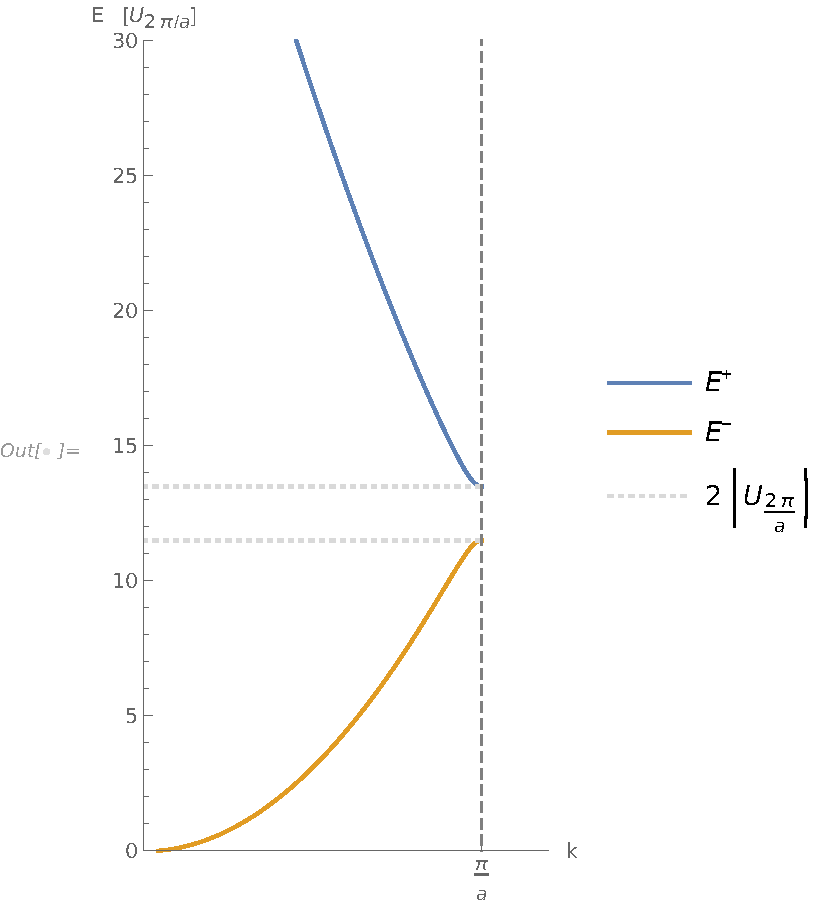
\includegraphics[trim=1.5cm 0 0 0,clip,width=0.4\textwidth]{5ai}
%		\caption{Equation~\refeq{Epm} as a function of $k$ with $\Epm$ in units of $\abs{\Utpa}$.  The top~(blue) curve corresponds to $\Ep$ and the bottom~(gold) curve to $\Em$.  The dark gray dashed line is the zone boundary at $k = K / 2 = \pi / a$.  The light gray dotted lines indicate the top and bottom of the gap, which has length $2 \abs{\Utpa}$.}
%	}
	
	At $k = \pi / a = K / 2$, the energy levels are given by (4.49) in the lecture notes,
	\eqn{4.49}{
		\Epm(K / 2) = \EohK \pm \abs{\UK}.
	}
	The leading corrections in $U$ for two energy levels are given by Ashcroft \& Mermin~(9.22),
	\al{
		(E - \Eok) \ck &= \UvK \ckmK, &
		(E - \EokmK) \ckmK &= \UmvK \ck
		= \UvKs \ck,
	}
	where $\ck$ and $\ckmK$ are the coefficients of the wavefunctions.  Substituting $k = \pi / a$ and $K = 2\pi / a$ andEq.~\refeq{4.49} into the first of these expressions, we find
	\eq{
		\Utpa \cpmkmpa = (\Epm - \Eopa) \cpmk
		= [ (\Eopa \pm \abs{\Utpa}) - \Eopa ] \cpmk
		= \pm \abs{\Utpa} \cpmk
	}
	which implies
	\eqn{ratio}{
		\ans{ \frac{\cpmk}{\cpmkmpa} = \pm \frac{\Utpa}{\abs{\Utpa}} }
	}
	as desired~\cite[p.~159]{Ashcroft}. \qed
	
}



\prob{
	Hence show that the probability density for the electronic states at $k = \pi / a$ take the form
	\al{
		\abs{\psipr}^2 &\propto \cos[2](\frac{\pi x}{a} + \frac{\phi}{2}), &
		\abs{\psimr}^2 &\propto \sin[2](\frac{\pi x}{a} + \frac{\phi}{2}).
	}
}

\sol{
	We assume the potential is attractive ($\UK < 0$).  The wavefunctions are given by (4.38) in the lecture notes,
	\eq{
		\psivkr = \sumK \ckmK e^{i (\vk - \vK) \vdot \vr}.
	}
	With $k = \pi / a$, this gives us
	\al{
		\psipr &= \cpk e^{i k x} + \cpkmpa e^{i (k - 2\pi / a) x}
		= \cpk (e^{i \pi x / a} - e^{-i \pi x / a})
		= 2 i \cpk \sin(\frac{\pi x}{a}), \\
		\psimr &= \cpk e^{i k x} + \cmkmpa e^{i (k - 2\pi /a) x}
		= \cpk (e^{i \pi x / a} + e^{-i \pi x / a})
		= 2 \cpk \cos(\frac{\pi x}{a}),
	}
	where we have used Eq.~\refeq{ratio}.  Then
	\al{
		\abs{\psipr}^2 &= -2 \abs{\cpk}^2 \sin[2](\frac{\pi x}{a})
		\propto \ans{ \cos[2](\frac{\pi x}{a} + \frac{\phi}{2}), } \\
		\abs{\psimr}^2 &= 2 \abs{\cpk}^2 \cos[2](\frac{\pi x}{a})
		\propto \ans{ \sin[2](\frac{\pi x}{a} + \frac{\phi}{2}), }
	}
	where we have included a phase shift $\phi / 2$ in order to account for the complex coefficient. \qed
}



\prob{
	Show that the potential can be written
	\eqn{Utpa}{
		\Utpa = \sin(\frac{\pi \del}{2}) \paren{ \UAtpa + \UBtpa } - i \cos(\frac{\pi \del}{2}) \paren{ \UAtpa - \UBtpa },
	}
	where
	\eq{
		\UABtpa = \frac{N}{V} \int \ddr e^{-2 \pi i r / a} \UABr.
	}
}

\sol{
	Since $\Ur$ is a sum of atomic potentials located at the positions of the atoms, it can be written as Ashcroft \& Mermin~(9.31):
	\eq{
		\Ur = \sumvR \brac{ \UA(\vr - \vR - \vdA) + \UB(\vr - \vR - \vdB) }
		= \sumvR \brac{ \UA\!\paren{ \vr - \vR - \frac{a}{4} (1 - \del) } + \UB\!\paren{ \vr - \vR + \frac{a}{4} (1 - \del) } },
	}
	where $\vdA$ and $\vdB$ are the positions of the atoms.  The momentum components of the potential are given by (4.20) in the lecture notes:
	\eq{
		\UvG = \frac{N}{V} \intuc \ddvr e^{-i \vG \vdot \vr} \Uvr.
	}
	Feeding in Eq.~\refeq{thing5c} and $K = 2 \pi / a$,
	\al{
		\UK &= \frac{N}{V} \intuc \ddr e^{-i K r} \sumR \brac{ \UA\!\paren{ r - R - \frac{a}{4} (1 - \del) } + \UB\!\paren{ r - R + \frac{a}{4} (1 - \del) } } \\
		&= \frac{N}{V} \brac{ \intas \ddr e^{-i K r} \UA\!\paren{ r - \frac{a}{4} (1 - \del) } + \intas \ddr e^{-i K r} \UB\!\paren{ r  + \frac{a}{4} (1 - \del) } }.
	}
	Let $r' = r \mp a (1 - \del) / 4$.  Then
	\eq{
		\UK = \frac{N}{V} \intas \ddrp e^{-i K r'} \brac{ e^{-i K a (1 - \del) / 4} \UArp + e^{-i K a (1 + \del) / 4} \UBrp }.
	}
	Renaming $r' \to r$ and applying $K = 2\pi / a$, we have
	\al{
		\Utpa &= \frac{N}{V} \intas \ddr e^{-i 2\pi r / a} \brac{ e^{-i 2\pi (1 - \del) / 4} \UAr + e^{-i 2\pi (1 + \del) / 4} \UBr } \\
		&= e^{-i \pi / 2} \frac{N}{V} \intas \ddr e^{-i 2\pi r / a} \brac{ e^{i \pi \del / 2} \UAr - e^{-i \pi \del / 2} \UBr } \\
		&= i \frac{N}{V} \brac{ \int \ddr e^{-i \pi (2 r / a + \del / 2)} \UBr - \int \ddr e^{-i \pi (2 r / a - \del / 2)} \UAr } \\
		&= i \frac{N}{V} \brac{ e^{-i \pi \del / 2} \int \ddr e^{-2 \pi i r / a} \UBr - e^{i \pi \del / 2} \int \ddr e^{-2 \pi i r / a} \UAr } \\
		&= i \brac{ e^{-i \pi \del / 2} \UBtpa - e^{i \pi \del / 2} \UAtpa } \\
		&= \frac{i}{2} \brac{ e^{-i \pi \del / 2} (\UAtpa + \UBtpa - \UAtpa + \UBtpa) - e^{i \pi \del / 2} (\UAtpa + \UBtpa + \UAtpa - \UBtpa) } \\
		&= \frac{i}{2} (e^{-i \pi \del / 2} - e^{i \pi \del / 2}) \paren{ \UAtpa + \UBtpa } - \frac{i}{2} (e^{-i \pi \del / 2} + e^{i \pi \del / 2}) \paren{ \UAtpa - \UBtpa } \\
		&= \ans{ \sin(\frac{\pi \del}{2}) \paren{ \UAtpa + \UBtpa } - i \cos(\frac{\pi \del}{2}) \paren{ \UAtpa - \UBtpa } }
	}
	as we wanted to show. \qed
}



\prob{
	The system contains an average of one electron per atom, or equivalently two electrons per unit cell.  Discuss the values of the energy gaps and plot the charge densities corresponding to the highest filled electron state and the lowest empty electron state in the two cases:
	\begin{enumerate}
		\item $\del = 0$, $\UsA \neq \UsB$;
		\item identical atoms, $\UsA = \UsB$, and $\del \neq 0$.
	\end{enumerate}
	Explain how this provides a simple model of either an \emph{ionic} or \emph{covalent} solid.
}

\sol{
	We know that the energy gap is $2 \abs{\Utpa}$.  In the first case, substituting $\del = 0$ into Eq.~\refeq{Utpa} gives us
	\eq{
		\Utpa = \sin(0) \paren{ \UAtpa + \UBtpa } - i \cos(0) \paren{ \UAtpa - \UBtpa }
		= -i \paren{ \UAtpa - \UBtpa }
	}
	so the energy gap is
	\eq{
		2 \abs{\Utpa} = \ans{ 2 \abs{ \UAtpa - \UBtpa }. }
	}
	This is small only if $\UA \approx \UB$.
	
	In the second case, substituting $\UsA = \UsB$ into Eq.~\refeq{Utpa} yields
	\eq{
		\Utpa = \sin(\frac{\pi \del}{2}) \paren{ \UAtpa + \UAtpa } - i \cos(\frac{\pi \del}{2}) \paren{ \UAtpa - \UAtpa }
		= 2 \sin(\frac{\pi \del}{2}) \UAtpa,
	}
	so the energy gap is
	\eq{
		2 \abs{\Utpa} = \ans{ 4 \abs{ \sin(\frac{\pi \del}{2}) \UAtpa }. }
	}
	Assuming $\del$ is small, this is close to 0.
	
	\hl{how to draw the things}	
%	delta is small, smaller band gap, metal/ionic
}



\state{Tight binding for BCC and FCC lattices}{
	Show that the tight-binding band structure for a body-centered cubic lattice (include only the hopping to the eight nearest neighbors) is
	\eq{
		\Evk = \epso + 8 t \cos(\frac{\kx a}{2}) \cos(\frac{\ky a}{2}) \cos(\frac{\kz a}{2}), 
	}
	and for the face-centered cubic lattice (twelve nearest neighbors)
	\eq{
		\Evk = \epso + 4 t \brac{ \cos(\frac{\kx a}{2}) \cos(\frac{\ky a}{2}) + \cos(\frac{\kx a}{2}) \cos(\frac{\ky a}{2}) + \cos(\frac{\kz a}{2}) \cos(\frac{\kx a}{2}) }.
	}
}

\sol{
	The band energy in the tight-binding description is given by (4.57) in the lecture notes,
	\eq{
		\Evk = \epso + t \sumrho e^{-i \vk \vdot \vrho}.
	}

	In a BCC lattice of spacing $a$, the eight nearest neighbors of the origin are located at
	\eq{
		\vrho \in \frac{a}{2} \{ (1, 1, 1),\ (-1, -1, -1),\ (1, 1, -1),\ (-1, -1, 1),\ (1, -1, 1),\ (-1, 1, -1),\ (-1, 1, 1),\ (1, -1, -1) \}.
	}
	So the band energy is
	\al{
		\Evk &= \epso + t \left( e^{-i a (\kx + \ky + \kz) / 2} + e^{-i a (-\kx - \ky - \kz) / 2} + e^{-i a (\kx + \ky - \kz) / 2} + e^{-i a (-\kx - \ky + \kz) / 2} \right. \\
		&\hspace{5em} \left. \phantom{=\ } + e^{-i a (\kx - \ky + \kz) / 2} + e^{-i a (-\kx + \ky - \kz) / 2} + e^{-i a (-\kx + \ky + \kz)} / 2 + e^{-i a (\kx - \ky - \kz) / 2} \right) \\[.5ex]
		&= \epso + t \paren{ e^{-i a \kx / 2} + e^{i a \kx / 2} } \paren{ e^{-i a \ky / 2} + e^{i a \ky / 2} } \paren{ e^{-i a \kz / 2} + e^{i a \kz / 2} } \\[.5ex]
		&= \epso + t \brac{ 2 \cos(\frac{\kx a}{2}) } \brac{ 2 \cos(\frac{\ky a}{2}) } \brac{ 2 \cos(\frac{\kz a}{2}) } \\[.5ex]
		&= \ans{ \epso + 8 t \cos(\frac{\kx a}{2}) \cos(\frac{\ky a}{2}) \cos(\frac{\kz a}{2}) }
	}
	as we wanted to show. \qed

	In an FCC lattice of spacing $a$, the twelve nearest neighbors of the origin are located at~\cite[p.~182]{Ashcroft}
	\al{
		\vrho &\in \frac{a}{2} \{ (1, 1, 0),\ (-1, -1, 0),\ (1, -1, 0),\ (-1, 1, 0),\ (1, 0, 1),\ (-1, 0, -1), \\
		&\hspace{5em} (1, 0, -1),\ (-1, 0, 1),\ (0, 1, 1),\ (0, -1, -1),\ (0, 1, -1),\ (0, -1, 1) \}.
	}
	So the band energy is
	\al{
		\Evk &= \epso + t \left( e^{-i a (\kx + \ky) / 2} + e^{-i a (-\kx - \ky) / 2} + e^{-i a (\kx - \ky) / 2} + e^{-i a (-\kx + \ky) / 2} \right. \\
		&\hspace{5em} \phantom{=\ } + e^{-i a (\kx + \kz) / 2} + e^{-i a (-\kx - \kz) / 2} + e^{-i a (\kx - \kz)} / 2 + e^{-i a (-\kx + \kz) / 2} \\
		&\hspace{10em} \left. \phantom{=\ } + e^{-i a (\ky + \kz) / 2} + e^{-i a (-\ky - \kz) / 2} + e^{-i a (\ky - \kz)} / 2 + e^{-i a (-\ky + \kz) / 2} \right) \\[.5ex]
		&= \epso + t \left[ \paren{ e^{-i a \kx / 2} + e^{i a \kx - / 2} } \paren{ e^{-i a \ky / 2} + e^{i a \ky / 2} } + \paren{ e^{-i a \kx / 2} + e^{i a \kx - / 2} } \paren{ e^{-i a \kz / 2} + e^{i a \kz / 2} } \right. \\
		&\hspace{5em} \left. \phantom{=\ } + \paren{ e^{-i a \ky / 2} + e^{i a \ky - / 2} } \paren{ e^{-i a \kz / 2} + e^{i a \kz / 2} } \right] \\[.5ex]
		&= \epso + t \curly{ \brac{ 2 \cos(\frac{\kx a}{2}) } \brac{ 2 \cos(\frac{\ky a}{2}) } + \brac{ 2 \cos(\frac{\kx a}{2}) } \brac{ 2 \cos(\frac{\kz a}{2}) } + \brac{ 2 \cos(\frac{\ky a}{2}) } \brac{ 2 \cos(\frac{\kz a}{2}) } } \\[.5ex]
		&= \ans{ \epso + 4 t \brac{ \cos(\frac{\kx a}{2}) \cos(\frac{\ky a}{2}) + \cos(\frac{\kx a}{2}) \cos(\frac{\ky a}{2}) + \cos(\frac{\kz a}{2}) \cos(\frac{\kx a}{2}) } }
	}
	as desired. \qed
}



\state{Pseudopotential}{
	Show that $\bkchifn = 0$ if we choose $\betn = \bkfnk$.
	
	The pseudopotential is not unique.  Show that the valence eigenvalues of a Hamiltonian $H + \VR$ are the same for any operator of the form
	\eq{
		\VR \kphi = \sumn \bkFnphi \kfn,
	}
	where the $\Fn$ are \emph{arbitrary} functions.
}

\sol{
	Equation~(4.59) of the lecture notes defines the basis vectors
	\eq{
		\kchivk = \kvk - \sumn \betn \kfnvk.
	}
	If we choose $\betn = \bkfnk$ and multiply on the left by $\bfn$, then
	\eq{
		\bkfnchi = \bkfnk - \summ \bkfmk \bkfnfm
		= \bkfnk - \summ \bkfmk \delmn
		= \bkfnk - \bkfnk
		= 0.
	}
	Since $\bkchifn = \bkfnchi^*$, we have shown that if $\betn = \bkfnk$ then
	\eq{
		\ans{ \bkchifn = 0 }
	}
	as desired. \qed
	
	For the valence eigenvalues,
	\eq{
		(H + \VR) \kphi
		= H \kphi + \sumn \bkFnphi \kfn
	}
	\hl{then idk what to do next}
}



\state{Hartree--Fock theory for the two-level atom}{
	Show that the Hartree--Fock total energy Eq.~(4.83) applied to the two-level atom model of Sec.~4.2.1 gives exactly the direct and exchange energy calculated in Eq.~(4.75).
}

\sol{
	Equation~(4.83) is
	\eq{
		\evHsPsi = \sumi \ev*{(T + \Uion)}{i} + \frac{1}{2} \sumij \paren{ \ev*{\frac{e^2}{\rij}}{i j} - \mel*{i j}{\frac{e^2}{\rij}}{j i} \delsigij }.
	}
	For the two-level atom, $i, j \in \{ 1, 2 \}$.  So we have
	\aln{
		\evHsPsi &= \ev*{(T + \Uion)}{1} + \ev*{(T + \Uion)}{2} \notag \\
		&\hspace{5em} \phantom{=\ }+ \frac{1}{2} \paren{ \ev*{\frac{e^2}{\rqw}}{1 2} - \mel*{1 2}{\frac{e^2}{\rqw}}{2 1} \delsigqw + \ev*{\frac{e^2}{\rwq}}{2 1} - \mel*{2 1}{\frac{e^2}{\rwq}}{1 2} \delsigqw }. \label{evHPsi}
	}
	since $\delsigii = 1$.

	Using (4.76) in the lecture notes, the direct energy is
	\eq{
		\ev{V}{1 2} = \ev*{\frac{e^2}{\rqw}}{1 2}
		= \int \ddvr \ddvrp \abs{\psiqrp}^2 \frac{e^2}{\absrmrp} \abs{\psiwr}^2
		= \int \ddvrp \ddvr \abs{\psiqr}^2 \frac{e^2}{\absrmrp} \abs{\psiwrp}^2
		= \ev*{\frac{e^2}{\rwq}}{2 1},
	}
	where we have simply interchanged $\vr$ and $\vr'$.  Similarly, using (4.77) in the lecture notes, the exchange energy is
	\al{
		\mel{2 1}{V}{1 2} &= \mel*{2 1}{\frac{e^2}{\rwq}}{1 2} \\
		&= \int \ddvr \ddvrp \psiwsr \psiqsrp \frac{e^2}{\absrmrp} \psiqr \psiwrp \\
		&= \int \ddvrp \ddvr \psiwsrp \psiqsr \frac{e^2}{\absrmrp} \psiqrp \psiwr \\
		&= \mel*{1 2}{\frac{e^2}{\rqw}}{2 1}.
	}
	From p.~53 of the lecture notes, $\Ei = \ev{(T + \Uion)}{i}$.  Finally, Eq.~\refeq{evHPsi} can be written
	\eq{
		\ans{ \evHPsi = \Eq + \Ew + \ev{V}{12} + \mel{21}{V}{12} }
	}
	which has the same direct and exchange energy as (4.75) in the lecture notes. \qed
}



\state{Hartree--Fock equations}{
	Evaluate the energy in the form
	\eq{
		\evHsPsi = \frac{\evHPsi}{\bkPsi}
	}
	with the determinantal wavefunction of Eq.~(4.82) using an orthonormal set of orbitals $\psii$.
	
	Show that by minimizing with respect to the $\psiis$ one obtains the Hartree--Fock equations
	\eq{
		\paren{ -\frac{\hbar^2}{2 m} \laplacian + \Uionr + \Ucoulr } \psiir - \sumj \int \ddvrp \frac{e^2}{\absrmrp} \psijsrp \psiirp \psijr \delsigij = \epsi \psiir,
	}
	and that the total energy can be written
	\eq{
		\evHsPsi = \sumi \epsi - \frac{1}{2} \sumij \paren{ \ev*{\frac{e^2}{\rij}}{i j} - \mel*{i j}{\frac{e^2}{\rij}}{j i} \delsigij }.
	}
}

\sol{
	Equation (4.82) of the lecture notes is
	\eq{
		\PsiHF = \mqty|
			\psiq(\vrq, \sigq) & \cdots & \psiq(\vrN, \sigN) \\
			\vdots & & \vdots \\
			\psiN(\vrq, \sigq) & \cdots & \psiN(\vrN, \sigN)
		|
	}
	
	Answer:
	\eq{
		\ans{ \evHsPsi = \sumi \ev*{T + \Uion}{i} + \frac{1}{2} \sumij \paren{ \ev*{\frac{e^2}{\rij}}{i j} - \mel*{i j}{\frac{e^2}{\rij}}{j i} \delsigij }. }
	}
	
	\hl{what the heck}
}







\state{Band structure in the Hartree--Fock approximation}{
	Using Eq.~(4.91), calculate the density of states near the Fermi energy to leading order in $(E - \EF) / \EF$.  If this result were physically correct, what would be the temperature dependence of the electronic specific heat at low temperature?
}

\sol{
	Equation~(4.91) from the lecture notes is
	\eq{
		\epsk = \frac{\hbar^2 k^2}{2 m} - \frac{2 e^2 \kF}{\pi} F(k / \kF)
	}
	where by (4.92),
	\eq{
		\Fx = \frac{1}{2} + \frac{1 - x^2}{4x} \ln\abs{ \frac{1 + x}{1 - x} }.
	}
	Making this substitution gives us
	\eqn{epsk}{
		\epsk = \frac{\hbar^2 k^2}{2 m} - \frac{2 e^2 \kF}{\pi} \paren{ \frac{1}{2} + \frac{1 - k^2 / \kF^2}{4 k / \kF} \ln\abs{ \frac{1 + k / \kF}{1 - k / \kF} } }
	}
	
	Then $\EF = \epsFk$ is
	\eq{
		\EF = \frac{\hbar^2 \kF^2}{2 m} - \frac{2 e^2 \kF}{\pi} \paren{ \frac{1}{2} + \frac{1 - \kF^2 / \kF^2}{4 \kF / \kF} \ln\abs{ \frac{1 + \kF / \kF}{1 - \kF / \kF} } }
		= \frac{\hbar^2 \kF^2}{2 m} - \frac{e^2 \kF}{\pi},
	}
	so
	\eq{
		\frac{E - \EF}{\EF} = \frac{\dfrac{\hbar^2 k^2}{2 m} - \dfrac{2 e^2 \kF}{\pi} F(k / \kF)}{\dfrac{\hbar^2 \kF^2}{2 m} - \dfrac{e^2 \kF}{\pi}} - 1
		= \frac{\dfrac{\hbar^2}{2 m} \paren{ \dfrac{k}{\kF} }^2 - \dfrac{2 e^2}{\pi \kF} F(k / \kF)}{\dfrac{\hbar^2}{2 m} - \dfrac{e^2}{\pi \kF}} - 1.
	}
	The first term will be close to 1, and thus $(E - \EF) / \EF$ will be very small, when $x = k / \kF \to 1$.
	
	From (4.34), the density of states can be found by
	\eq{
		\gE = 2 \frac{4\pi k^2}{(2\pi)^3 / V} \dv{k}{E}.
	}
	From our Eq.~\refeq{epsk}, we have
	\eq{
		\dv{E}{k} = \frac{\hbar^2}{m} k - \frac{e^2 \kF}{\pi k} + \frac{e^2}{2\pi} \paren{ 1 + \frac{\kF^2}{k^2} } \ln\abs{\frac{1 + k / \kF}{1 - k / \kF}}.
	}
	Then the density of states is
	\al{
		\gE &= 2 \frac{4\pi k^2}{(2\pi)^3 / V} \brac{ \frac{\hbar^2}{m} k - \frac{e^2 \kF}{\pi k} + \frac{e^2}{2\pi} \paren{ 1 + \frac{\kF^2}{k^2} } \ln\abs{\frac{1 + k / \kF}{1 - k / \kF}} }^{-1} \\
		&= \frac{\kF^2 V}{\pi^2} x^2 \brac{ \frac{\hbar^2 \kF}{m} x - \frac{e^2}{\pi} \frac{1}{x} + \frac{e^2}{2\pi} \paren{ 1 + \frac{1}{x^2} } \ln\abs{\frac{1 + x}{1 - x}} }^{-1} \\
		&\approx \frac{\kF^2 V}{\pi^2} \frac{m \pi}{-e^2 m + \pi \hbar^2 \kF + e^2 m \ln\abs{\dfrac{2}{1 - x}} } \\ %+ (x - 1) \frac{\pi m}{2} \frac{-7 e^2 m + 2 \pi \hbar^2 \kF + 5 e^2 m \ln\abs{\dfrac{2}{1 - x}}}{\paren{ -e^2 m + \pi \hbar^2 \kF + e^2 m \ln\abs{\dfrac{2}{1 - x}} }^2 } } \\
		&\approx \ans{ \frac{\kF^2 V}{\pi} \frac{m}{\pi \hbar^2 \kF + e^2 m \paren{ \ln\abs{\dfrac{2}{1 - k / \kF}} - 1 } }, }
	}
	where we have performed a Taylor series expansion to zeroth order using Mathematica.
	
	The specific heat can be calculated from Eq.~(2.15) in the lecture notes:
	\eq{
		\cv = \int \ddE E \gE \pdv{\fE}{T}.
	}
	Transforming this to an integral over $k$, we have
	\al{
		\cv &= \int \ddk \dv{E}{k} \epsk \paren{ 2 \frac{4\pi k^2}{(2\pi)^3 / V} \dv{k}{E} } \pdv{\fE}{T} \\
		&= \int \ddk \brac{ \frac{\hbar^2 k^2}{2 m} - \frac{2 e^2 \kF}{\pi} \paren{ \frac{1}{2} + \frac{1 - k^2 / \kF^2}{4 k / \kF} \ln\abs{ \frac{1 + k / \kF}{1 - k / \kF} } } } \brac{ 2 \frac{4\pi k^2}{(2\pi)^3 / V} } \pdv{\fE}{T}
	}
	From (2.17):
	\eq{
		\dv{f}{T} = \frac{e^y}{(e^y + 1)^2} \paren{ \frac{y}{T} + \frac{1}{\kB T} \dv{\mu}{T} }
		= \frac{e^y}{(e^y + 1)^2} \frac{y}{T}
	}
	where $y = (E - \mu) / \kB T$, and $\mu$ changes slowly at low temperature.  Note that
	\al{
		\exp(\frac{E - \mu}{\kB T}) &= \exp\!\curly{ \frac{1}{\kB T} \brac{ \frac{\hbar^2 k^2}{2 m} - \frac{2 e^2 \kF}{\pi} \paren{ \frac{1}{2} + \frac{1 - k^2 / \kF^2}{4 k / \kF} \ln\abs{ \frac{1 + k / \kF}{1 - k / \kF} } } - \mu } } \\
		&= \exp(\frac{\hbar^2 k^2}{2 m \kB T}) \exp(-\frac{e^2 \kF}{\pi \kB T}) \exp(- \frac{2 e^2 \kF}{\pi} \frac{1 - k^2 / \kF^2}{4 k / \kF} \ln\abs{ \frac{1 + k / \kF}{1 - k / \kF}} ) \exp(-\frac{\mu}{\kB T})
	}
	
	\hl{help}
	
	
}






\state{Ferromagnetism in the HF approximation}{
	Previously, we considered the unpolarized spin state, which is a paramagnet.  Now consider a fully spin polarized state at the same density: the Hartree--Fock Slater determinant corresponds to singly occupying each state in the  Fermi sphere.  In analogy to Eq.~(4.93), compute the total energy of the spin polarized state, and show that this is lower in energy than the unpolarized state if $\rs > 5.45$ in the Hartree--Fock approximation.
}






\state{Thomas--Fermi screening}{
	Check the formulae in Eq.~(4.133) and Eq.~(4.134).  Supposing that the potential $\vext = Q / r$, show that the induced charge density is then of the form
	\eq{
		\del\nr \propto \frac{e^{-r / \xi}}{r}
	}
	and identify the screening length $\xi$.
}

\sol{
	Equation~(4.133) is
	\eq{
		\del \nvq = -\frac{\vextvq}{\dfrac{4\pi e^2}{q^2} \paren{ 1 + \dfrac{q^2}{\qTF^2} }},
	}
	and (4.124) is
	\eq{
		\qTF^2 = \frac{4}{\pi} \frac{m e^2}{\hbar^2} \kF.
	}
	
	We must Fourier transform $\vext$ to get an expression in terms of $\vq$.  From Ashcroft \& Mermin~(17.52),
	\eq{
		\vextvr = \frac{Q}{r}
		\qimplies
		\vextvq = \frac{4\pi Q}{q^2}.
	}
	Then
	\eq{
		\del\nvq = \frac{4 \pi Q / q^2}{\dfrac{4\pi e^2}{q^2} \paren{ 1 + q^2 \dfrac{\pi}{4} \dfrac{\hbar^2}{m e^2 \kF} }}
		= \frac{4 \pi Q / q^2}{\dfrac{4\pi e^2}{q^2} + \dfrac{\pi^2 \hbar^2}{m \kF} }
		= \frac{Q}{e^2 + \dfrac{\pi \hbar^2}{4 m \kF} q^2 }.
	}
	The inverse Fourier transform is
	\al{
		\del\nr &= \int \frac{\ddvq}{(2\pi)^3} e^{-i \vq \vdot \vr} \frac{Q}{e^2 + \dfrac{\pi \hbar^2}{4 m \kF} \abs{\vq}^2} \\
		&= Q \int \frac{\ddq}{(2\pi)^3} \intopi \ddtht \intotp \ddphi e^{-i q r \cos\tht} \frac{q^2 \sin\tht}{e^2 + \dfrac{\pi \hbar^2}{4 m \kF} q^2} \\
		&= 4\pi Q \intoi \frac{\ddq}{(2\pi)^3} \frac{\sin(q r)}{q r} \frac{q^2}{e^2 + \dfrac{\pi \hbar^2}{4 m \kF} q^2} \\
		&= 4\pi \frac{Q}{r} \intoi \frac{\ddq}{(2\pi)^3} \frac{x \sin x}{e^2 r^2 + \dfrac{\pi \hbar^2}{4 m \kF} x^2} \\
		&= \frac{2\pi^2}{\pi \hbar^2 / 4 m \kF} \frac{Q}{(2\pi)^3 r} \exp(-\frac{e r}{\sqrt{\pi \hbar^2 / 4 m \kF}}) \\
		&= \ans{ \frac{m \kF Q}{\pi^2 \hbar^2} \frac{1}{r} \exp(-\frac{r}{\qTF}) }
	}
	where we have defined $x = q r$.  Then \ans{$\xi = \qTF$}. \qed
}






\state{Generalized one-dimensional band theory}{
	Consider a 1D solid, lattice constant $a$, made of ``building blocks'' ($-a / 2< x < a / 2$) that scatter plane waves with a reflection coefficient $r$ and transmission coefficient $t$ ($\absr^2 + \abst^2 = 1$).  The energy of the plane wave is written as $\eps = \hbar^2 K^2 / 2 m$.  In the solid, the building blocks are stacked together indefinitely in the $x$ direction.
}

\prob{
	Write the solution to the {\Schrodinger} equation in the solid $\psix$, as a linear combination of $\psirx$ and $\psilx$ and use Bloch’s theorem to relate the wavefunction at each side of the building block (the same theorem applies to the gradient $\psi'$):
	\al{
		\psixpa &= e^{i k a} \psix, &
		\psipxpa &= e^{i k a} \psipx.
	}
	Hence, show
	\eq{
		\cos(k a) = \frac{t^2 - r^2}{2 t} e^{i K a} + \frac{1}{2 t} e^{-i K a}.
	}
}



\prob{
	If the transmission coefficient is $t = \abst e^{i \del}$, it can be shown that $r = \pm i \absr e^{i \del}$.  Use this result to eliminate $r$ and show
	\eq{
		\frac{\cos(k a + \del)}{\abst} = \cos(k a).
	}
	\vfix
}



\prob{
	Since $\abst < 1$, this result shows there are values of $K$ (and hence $\eps$) for which no Bloch states exist.  Demonstrate this by sketching the left-hand side as a function of $K$ (or preferably $\eps$).  Use your sketch to illustrate the behavior for
	\begin{enumerate}
		\item strong scattering, and
		\item weak scattering.
	\end{enumerate}
	Explain why, in general, electron bands tend to get wider and their gaps narrower as the electron energy increases.
}


\makebib
	
\end{document}
